\documentclass[noinstructornotes]{ximera}
%handout:  for handout version with no solutions or instructor notes
%handout,instructornotes:  for instructor version with just problems and notes, no solutions
%noinstructornotes:  shows only problem and solutions

%% handout
%% space
%% newpage
%% numbers
%% nooutcomes

%I added the commands here so that I would't have to keep looking them up
%\newcommand{\RR}{\mathbb R}
%\renewcommand{\d}{\,d}
%\newcommand{\dd}[2][]{\frac{d #1}{d #2}}
%\renewcommand{\l}{\ell}
%\newcommand{\ddx}{\frac{d}{dx}}
%\everymath{\displaystyle}
%\newcommand{\dfn}{\textbf}
%\newcommand{\eval}[1]{\bigg[ #1 \bigg]}

%\begin{image}
%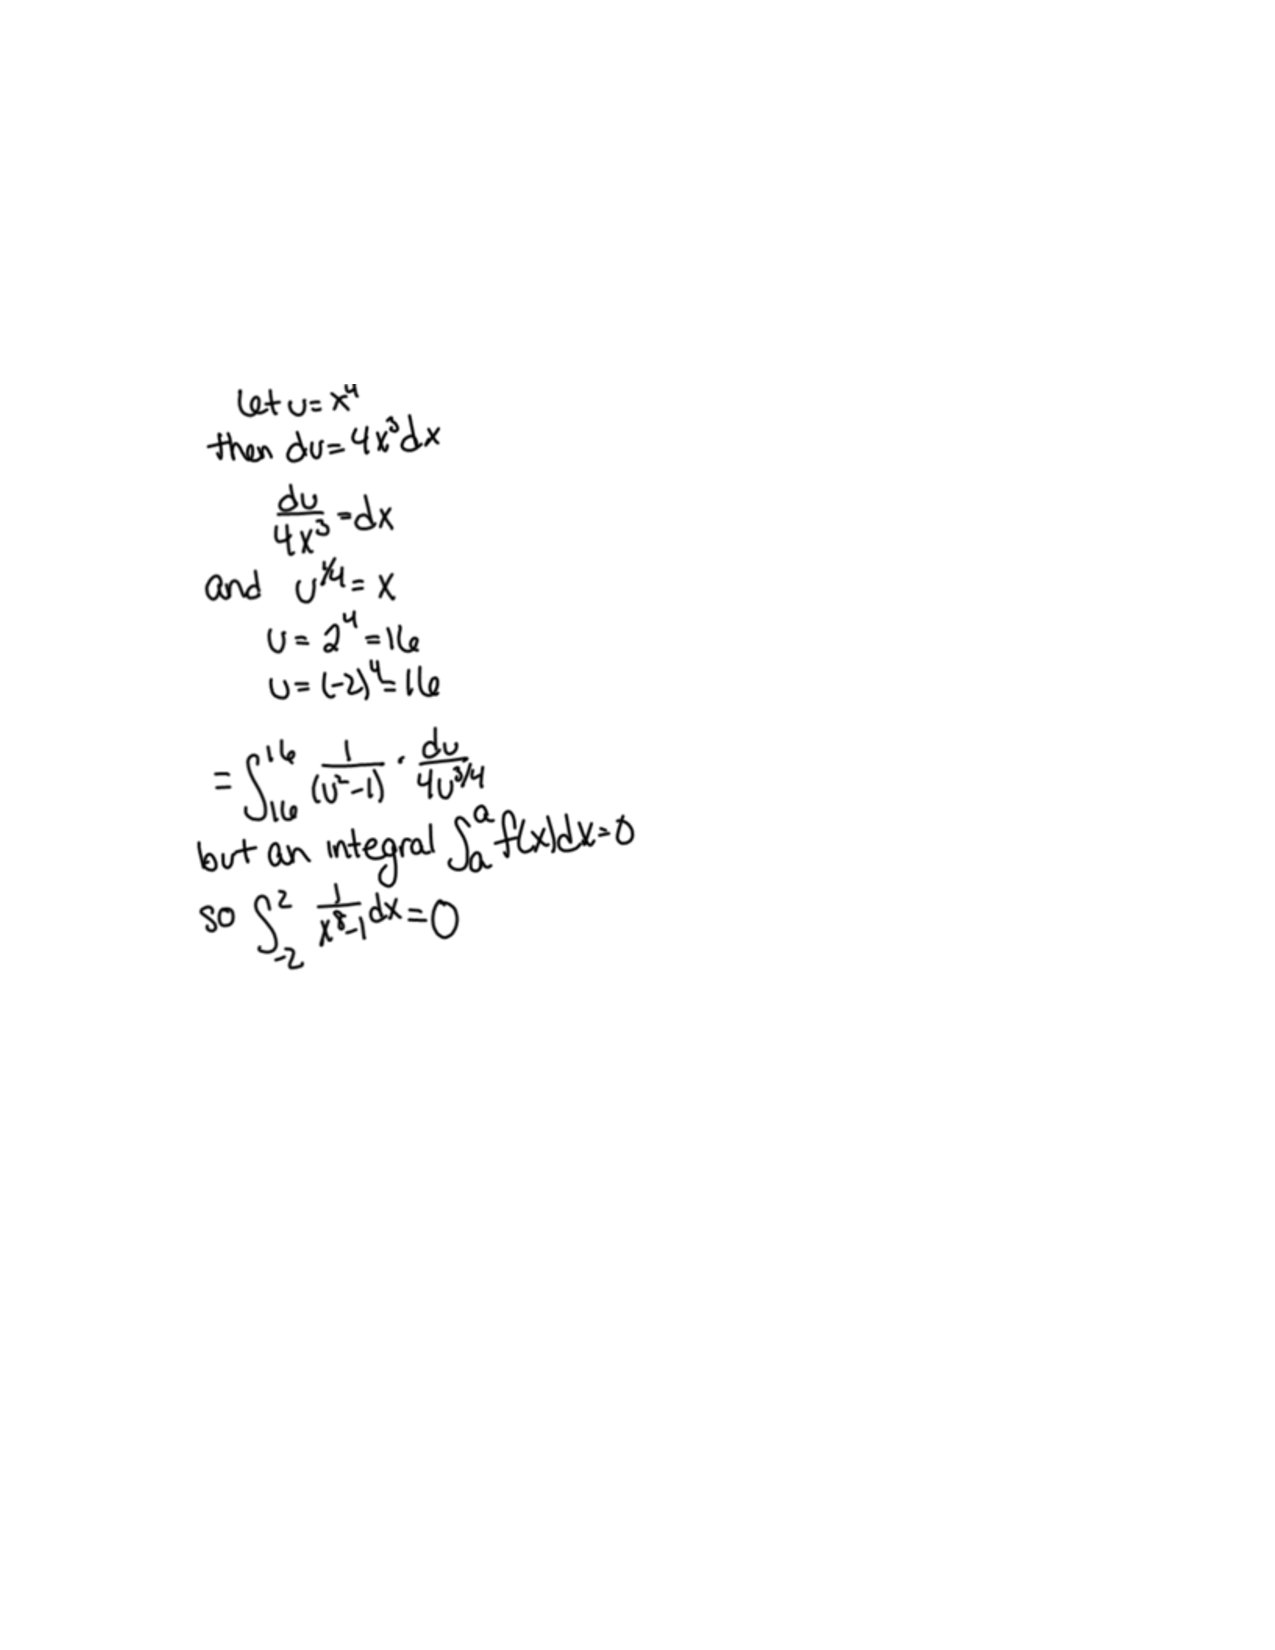
\includegraphics[trim= 170 420 250 180]{Figure1.pdf}
%\end{image}

%add a ``.'' below when used in a specific directory.
\newcommand{\RR}{\mathbb R}
\renewcommand{\d}{\,d}
\newcommand{\dd}[2][]{\frac{d #1}{d #2}}
\renewcommand{\l}{\ell}
\newcommand{\ddx}{\frac{d}{dx}}
\newcommand{\dfn}{\textbf}
\newcommand{\eval}[1]{\bigg[ #1 \bigg]}

\usepackage{multicol}

\renewenvironment{freeResponse}{
\ifhandout\setbox0\vbox\bgroup\else
\begin{trivlist}\item[\hskip \labelsep\bfseries Solution:\hspace{2ex}]
\fi}
{\ifhandout\egroup\else
\end{trivlist}
\fi} %% we can turn off input when making a master document

%\usepackage{fullpage}

\title{Recitation \#9: Trig Integrals and Trig Substitution}  

\begin{document}
\begin{abstract}		\end{abstract}
\maketitle



\begin{comment}
\section{Warm up:}

	\begin{freeResponse}
	
	\end{freeResponse}
	
\begin{instructorNotes}

\end{instructorNotes}
\end{comment}







\section{Group work:}


%problem 1
\begin{problem}
Evaluate the following integrals
	\begin{enumerate}
	
	\item  $\int \tan^{23} x \sec^6 x \d x$
	\begin{freeResponse}
		\begin{align*}
		\int \tan^{23} x \sec^6 x \d x 
		&= \int \tan^{23} x \sec^4 x \sec^2 x \d x  \\
		&= \int \tan^{23} x \left( 1 + \tan^2 x \right)^2 \sec^2 x \d x .
		\end{align*}
	We now substitute
		{\color{red}
		\[
		u = \tan x 	\qquad	\Longrightarrow		\qquad	\d u = \sec^2 x \d x.
		\]
		}
	Then
		\begin{align*}
		\int \tan^{23} x \left( 1 + \tan^2 x \right)^2 \sec^2 x \d x
		&= \int u^{23} (1+u^2)^2 \d u  \\
		&= \int u^{23} (1 + 2u^2 + u^4) \d u  \\
		&= \int \left( u^{23} + 2u^{25} + u^{27} \right) \d u  \\
		&= \frac{1}{24} u^{24} + \frac{1}{13} u^{26} + \frac{1}{28} u^{28} + C  \\
		&= \frac{1}{24} \tan^{24} x + \frac{1}{13} \tan^{26} x + \frac{1}{28} \tan^{28} x + C.
		\end{align*}
	\end{freeResponse}
	
	
	
	\item  $\int \tan^2 x \sec x \d x$ \qquad {\color{red} Hint:  $\int \sec x \d x = \ln | \sec x \tan x| + C$}
	\begin{freeResponse}
		\begin{align}
		\int \tan^2 x \sec x \d x
		&= \int \left( \sec^2 x - 1 \right) \sec x \d x  \nonumber	\\
		&= \int \sec^3 x \d x - \int \sec x \d x  		\nonumber	\\
		&= \int \sec^3 x \d x - \ln | \sec x \tan x| 	\qquad	{\color{red}\text{from the hint}}	\label{equation 1}
		\end{align}
	Now, in an attempt to evaluate $\int \sec^3 x \d x$, we use integration by parts with
		{\color{red}
		\[
		u = \sec x 				\qquad	\d v = \sec^2 x \d x
		\]
		\[
		\d u = \sec x \tan x \d x	\qquad	v = \tan x.
		\]
		}
	So
		\begin{equation}\label{equation 2}
		\int \sec^3 x \d x = \sec x \tan x - \int \tan^2 x \sec x \d x.
		\end{equation}
	Combining equations \eqref{equation 1} and \eqref{equation 2} yields
		\begin{align*}
		\int \tan^2 x \sec x \d x &= \int \sec^3 x \d x - \ln | \sec x \tan x|   \\
		\int \tan^2 x \sec x \d x &= \sec x \tan x - \int \tan^2 x \sec x \d x - \ln | \sec x \tan x |  \\
		2 \int \tan^2 x \sec x \d x &= \sec x \tan x - \ln | \sec x \tan x | + C  \\
		\int \tan^2 x \sec x \d x &= \frac{1}{2} \left( \sec x \tan x - \ln | \sec x \tan x | \right) + C.
		\end{align*}
	\end{freeResponse}
	
	
	
	\item  $\int \tan^2 x \sin x \d x$
	\begin{freeResponse}
		\begin{align*}
		\int \tan^2 x \sin x \d x
		&= \int \frac{\sin^2 x}{\cos^2 x} \sin x \d x  \\
		&= \int \frac{1-\cos^2 x}{\cos^2 x} \sin x \d x.
		\end{align*}
	Now we substitute
		{\color{red}
		\[
		u = \cos x 		\qquad	\Longrightarrow		\qquad	\d u = - \sin x \d x, \quad - \d u = \sin x \d x.
		\]
		}
	This gives us that
		\begin{align*}
		\int \tan^2 x \sin x \d x
		&= \int \frac{1-u^2}{u^2} (-1) \d u  \\
		&= \int \frac{u^2 - 1}{u^2} \d u  \\
		&= \int \left( 1 - u^{-2} \right) \d u  \\
		&= u + \frac{1}{u} + C  \\
		&= \cos x + \sec x + C.
		\end{align*}
	\end{freeResponse}
	
	\end{enumerate}
	
\end{problem}

\begin{instructorNotes}
All three parts involve standard strategies learned in the online lessons.  
For each, split the problems between the groups.  
Then discuss each problem as a class, getting input from the group(s) that worked on that problem.
\end{instructorNotes}







%problem 2
\begin{problem}
Evaluate
	\[
	\int_{- \pi}^0 \sqrt{1 - \cos^2 x} \d x.
	\]
	\begin{freeResponse}
		\begin{align*}
		\int_{- \pi}^0 \sqrt{1 - \cos^2 x} \d x
		&= \int_{- \pi}^0 \sqrt{\sin^2 x} \d x  \\
		&= \int_{- \pi}^0 | \sin x | \d x.
		\end{align*}
	Now, when $-\pi \leq x \leq 0$, $\sin x \leq 0$.  
	Thus, on this region, $|\sin x | = - \sin x$.
	So we continue
		\begin{align*}
		\int_{- \pi}^0 \sqrt{1 - \cos^2 x} \d x
		&= \int_{- \pi}^0 - \sin x \d x  \\
		&= \eval{\cos x}_{-\pi}^0  \\
		&= \cos(0) - \cos(-\pi) = 1 - (-1) = 2.
		\end{align*}
	\end{freeResponse}
		
\end{problem}

\begin{instructorNotes}
You may want to do this problem as a whole class - perhaps play-acting by claiming that it is equal to $\int_{-\pi}^0 \sin x \d x$ rather than $\int_{-\pi}^0 \left| \sin x \right|  \d x$
\end{instructorNotes}



%problem 3
\begin{problem}
Evaluate the following integrals
	\begin{enumerate}
	\item 
	\[
	\int \limits_{ -\frac{5}{3}}^{-\frac{5}{6}} \frac{\sqrt{36x^2-25}}{x^3} \d x.
	\]
	\begin{freeResponse}
	First notice that
		\begin{align*}
		\sqrt{36x^2-25} &= 5\sqrt{\frac{36x^2}{25} - 1}  \\
		&= 5\sqrt{\left( \frac{6x}{5} \right)^2 - 1}.
		\end{align*}
	So we substitute
		\[
		\frac{6x}{5} = \sec \theta	\qquad	\Longrightarrow	\qquad	x = \frac{5}{6} \sec \theta
		\]
	which gives
		\[
		\d x = \frac{5}{6} \sec \theta \tan \theta \d \theta  .
		\]
	Also, notice that
		\begin{itemize}
		\item when $x = - \frac{5}{3}$:
			\[
			-\frac{5}{3} = \frac{5}{6} \sec \theta \qquad	\Longrightarrow \qquad 	\sec \theta = 2 	\qquad 	\Longrightarrow 	\qquad	\theta = \frac{2\pi}{3}
			\]
			
		\item and when $x=-\frac{5}{6}$:\
			\[
			-\frac{5}{6} = \frac{5}{6} \sec \theta	\qquad	\Longrightarrow	\qquad	\sec \theta = -1	\qquad	\Longrightarrow	\qquad	\theta = \pi.
			\]
		\end{itemize}

	Therefore
		\begin{align*}
		\int_{-\frac{5}{3}}^{-\frac{5}{6}} \frac{\sqrt{36x^2-25}}{x^3} \d x 
		&= 5 \int_{\frac{2\pi}{3}}^{\pi} \frac{\sqrt{\sec^2 \theta - 1}}{\left( \frac{5}{6} \sec \theta \right)^3} \left( \frac{5}{6} \sec \theta \tan \theta \right) \d \theta  \\
		&= 5 \cdot \left(\frac{6}{5} \right)^2 \int_{\frac{2\pi}{3}}^{\pi} \frac{|\tan \theta| \tan \theta}{\sec^2 \theta} \d \theta .
		\end{align*}
	Now, notice that $\tan \theta < 0$ whenever $\frac{2\pi}{3} \leq \theta \leq \pi$.  
	So $|\tan \theta| = - \tan \theta$.
	We continue:
		\begin{align*}
		5 \cdot \left(\frac{6}{5} \right)^2 \int_{\frac{2\pi}{3}}^{\pi} \frac{|\tan \theta| \tan \theta}{\sec^2 \theta} \d \theta
		&= - \frac{36}{5} \int_{\frac{2\pi}{3}}^{\pi} \frac{\tan^2 \theta}{\sec^2 \theta} \d \theta  \\
		&= - \frac{36}{5} \int_{\frac{2\pi}{3}}^{\pi} \frac{\sin^2 \theta}{\cos^2 \theta} \cdot \frac{\cos^2 \theta}{1} \d \theta  \\
		&= - \frac{36}{5} \int_{\frac{2\pi}{3}}^{\pi} \sin^2 \theta \d \theta  \\
		&= - \frac{36}{5} \int_{\frac{2\pi}{3}}^{\pi} \frac{1}{2} \left( 1 - \cos (2\theta) \right) \d \theta  \\
		&= - \frac{18}{5} \eval{\theta - \frac{1}{2} \sin (2\theta)}_{\frac{2\pi}{3}}^{\pi}  \\
		&= - \frac{18}{5} \left[ \left( \pi - 0 \right) - \left( \frac{2\pi}{3} + \frac{\sqrt{3}}{4} \right) \right]  
		\qquad {\color{red} \sin \left( \frac{4\pi}{3} \right) = -\frac{\sqrt{3}}{2} }\\
		&= - \frac{18}{5} \left( \frac{\pi}{3} - \frac{\sqrt{3}}{4} \right).
		\end{align*}
	\end{freeResponse}
	
	\item 
	\[
	\int \frac{\d x}{\left( x^2 - 6x + 11 \right)^2}.
	\]
	\begin{freeResponse}
	We begin by completing the square in the denominator
		\[
		x^2 - 6x - 11 = x^2 - 6x + 9 + 2 = (x-3)^2 + 2.
		\]
	We then have that
		\begin{align*}
		\int \frac{\d x}{\left( x^2 - 6x + 11 \right)^2} 
		&= \int \frac{1}{((x-3)^2 + 2)^2} \d x  \\
		&= \frac{1}{4} \int \frac{1}{\left( \frac{(x-3)^2}{2} + 1 \right)^2} \d x  \\
		&= \frac{1}{4} \int \frac{1}{\left( \left( \frac{x-3}{\sqrt{2}} \right)^2 + 1 \right)^2} \d x.
		\end{align*}
	So we substitute
		\begin{equation}\label{substitution1}
		\frac{x-3}{\sqrt{2}} = \tan \theta	\qquad	\Longrightarrow	\qquad	x = \sqrt{2} \tan \theta + 3
		\end{equation}
	and then
		\[
		\d x = \sqrt{2} \sec^2 \theta \d \theta.
		\]
	Continuing with the integral
		\begin{align*}
		\frac{1}{4} \int \frac{1}{\left( \left( \frac{x-3}{\sqrt{2}} \right)^2 + 1 \right)^2} \d x
		&= \frac{1}{4} \int \frac{1}{\left( \tan^2 \theta + 1 \right)^2} \sqrt{2} \sec^2 \theta \d \theta  \\
		&= \frac{\sqrt{2}}{4} \int \frac{1}{\sec^2 \theta} \d \theta  \\
		&= \frac{\sqrt{2}}{4} \int \cos^2 \theta \d \theta  \\
		&= \frac{\sqrt{2}}{4} \int \frac{1}{2} \left( 1 + \cos(2\theta) \right) \d \theta  \\
		&= \frac{\sqrt{2}}{8} \left( \theta + \frac{1}{2} \sin(2\theta) \right) + C .
		\end{align*}
	Now all that is left to do is to reverse-substitute for $\theta$.  
	First, from equation \eqref{substitution1} we have that
		\[
		\theta = \arctan \left( \frac{x-3}{\sqrt{2}} \right).
		\]
	Now, we again use equation \eqref{substitution1} along with Pythagorean's Theorem to construct the following triangle.
	
		\begin{image}
		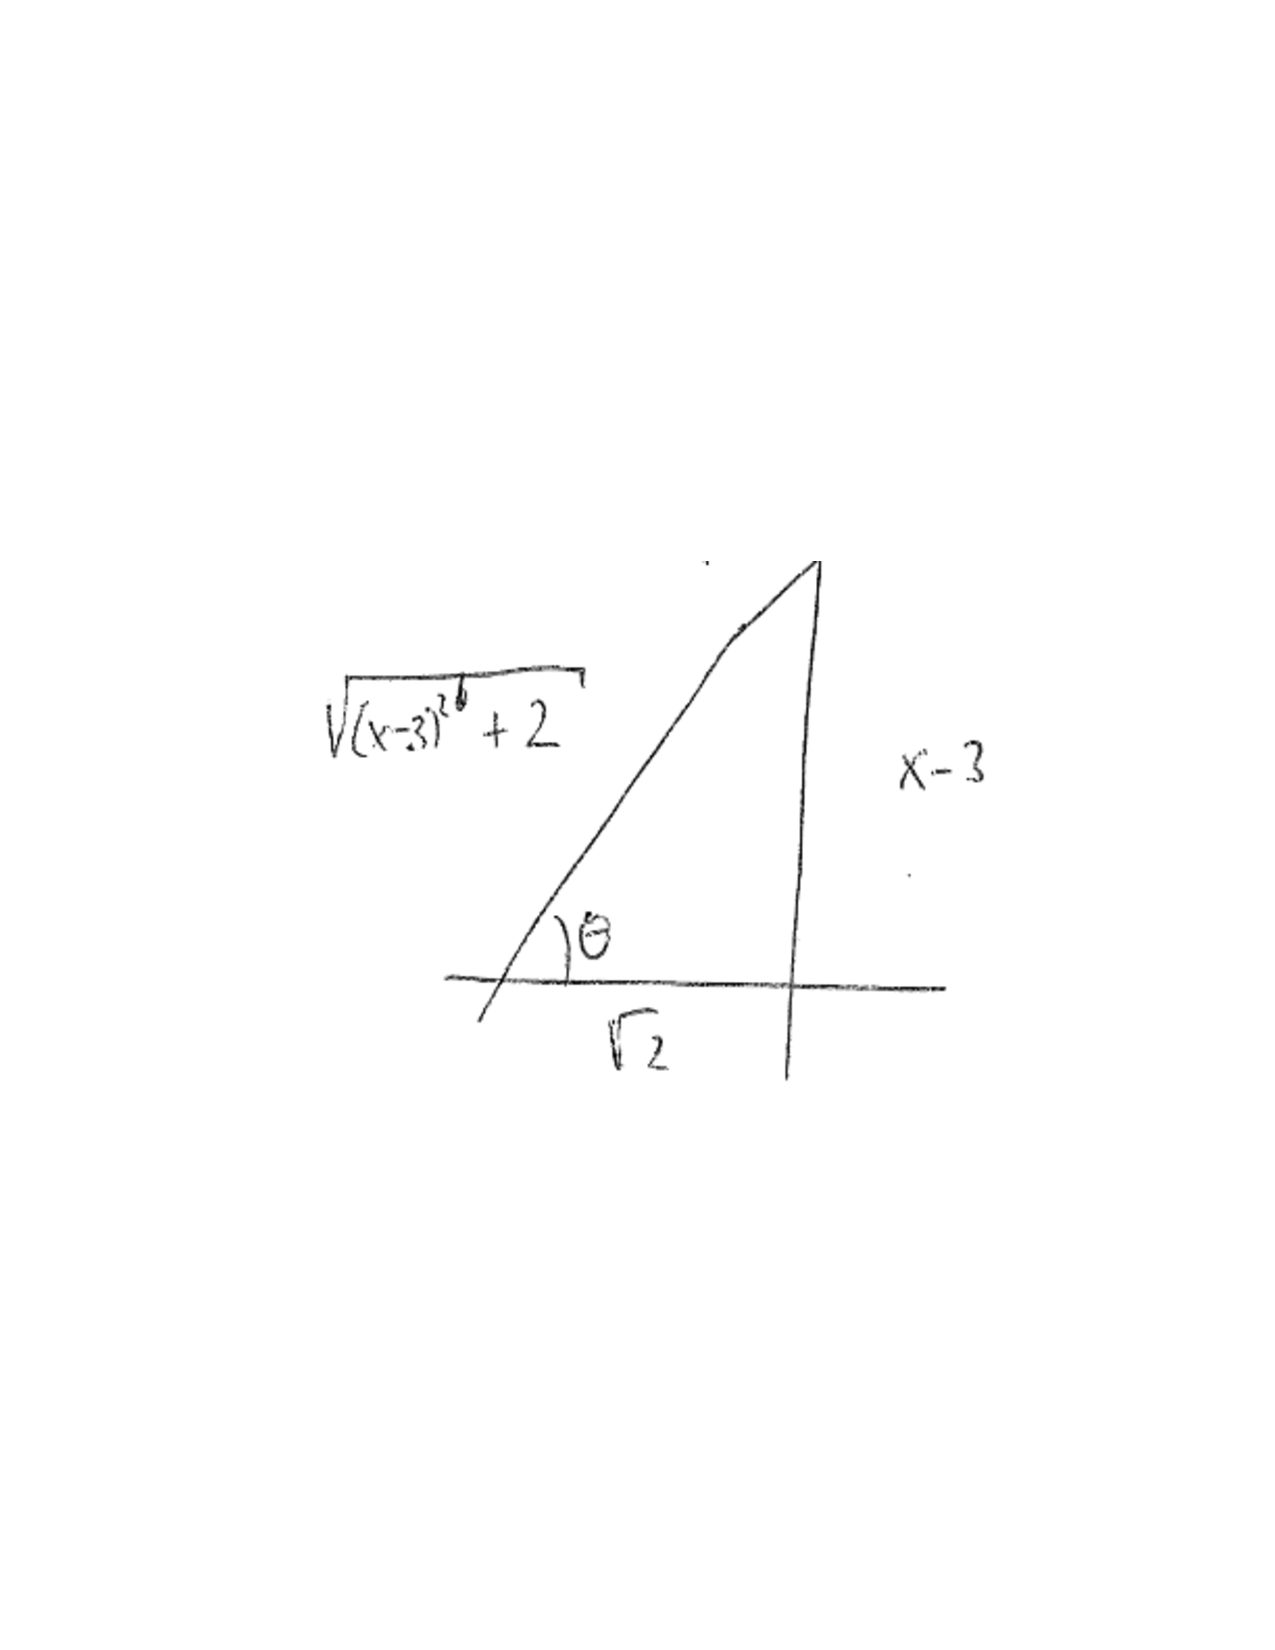
\includegraphics[trim= 230 270 250 280, scale=0.8]{Figure7-4-1.pdf}
		\end{image}
		
	Then we have that
		\[
		\sin(2\theta) = 2 \sin(\theta) \cos(\theta) = 2 \cdot \frac{x-3}{\sqrt{(x-3)^2+2}} \cdot \frac{\sqrt{2}}{\sqrt{(x-3)^2+2}}.
		\]
	Thus
		\[
		\int \frac{\d x}{\left( x^2 - 6x + 11 \right)^2} = \frac{\sqrt{2}}{8} \left( \arctan \left( \frac{x-3}{\sqrt{2}} \right) + \frac{\sqrt{2}(x-3)}{(x-3)^2+2} \right) + C .
		\]
	\end{freeResponse}
		


	\end{enumerate}

\end{problem}

\begin{instructorNotes}
Each of problems (a) through (c) involves one or more of the major points of trig substitution.  
Each of the three kinds of substitutions is represented, as well as working with absolute value issues in problem (a) (also could be brought up in problem (c)), completing the square, back substitution (c), and various trigonometric integrals.  
\dfn{Be adamant about substituting for $\d x$} as well as the rest of the integrand.  
In  (a), show the time-saving value of changing the limits in terms of $\theta$.  
\end{instructorNotes}















	
	
	
	
	
	
	
	
	

	










								
				
				
	














\end{document} 


















